% encoding utf8
% loot at the auml: ä

\documentclass[11pt, a4paper]{article}

\usepackage[T1]{fontenc}
\usepackage[utf8]{inputenc}
\usepackage[english]{babel}
\usepackage{makeidx} %Zur automatischen Indexerstellung
\usepackage{amsfonts}
\usepackage{amssymb}
\usepackage{epsfig}   % Zum Einbinden von Bildern
\usepackage{url}      % Korrekter Satz von URLs    
\usepackage[table,dvipsnames]{xcolor}    % Verwendung von Farben
\usepackage{colortbl}
\usepackage{footnote}
\usepackage{listings} % Korrekter Satz von Listings und Quellcode
\usepackage{fancyvrb}
\usepackage{color}
%\usepackage{algpseudocode}
%\usepackage{algorithm}
%\usepackage{mathptmx}			% Times/Mathe \rmdefault
%\usepackage[scaled=.90]{helvet}	% Skalierte Helvetica \sfdefault
%\usepackage{courier}			% Courier \ttdefault
%\usepackage{booktabs}
%\usepackage{pgfplots}
%\usepackage{tablefootnote}
%\pgfplotsset{compat=1.8}
%\usepackage{longtable}
\usepackage{fancyhdr}


% Zusatzpakete für mehr mathematische Symbole, Einfügen von Grafiken 
% und bessere Bildunterschriften
\usepackage{amsmath,amsthm,amsfonts,graphicx,caption}
\usepackage{subcaption}

\newtheorem{exmp}{Example}[section]


% set up caption style
\captionsetup{margin=10pt,font=small,labelfont=bf,format=hang}

% avoid single lines at beginning/end of page
\clubpenalty=10000
\widowpenalty=10000
\hyphenation{}

% Wenn man direkt mit dem pdflatex eine PDF-Datei erzeugt, sollten diese beiden
% Pakete eingebunden werden (Hyperlinks, bessere Bildschirmschriftarten usw.)
% Optionen zu den farbigen Rahmen von Links in eckigen Klammern.
\usepackage[colorlinks=false, pdfborder={0 0 0}, pdfborderstyle={/S/U/W 1}]{hyperref}

\usepackage{ae,aecompl}

%\usepackage[nonumberlist,toc]{glossaries}
%\newglossary[slg1]{roman}{syi1}{syg1}{roman}
%\makeglossaries


% author at the side of a section etc.
\newcommand{\sauth}[1]{\marginpar{\hspace{0.25cm}\textit{\scriptsize #1}}}


\lstset{basicstyle=\ttfamily} % fixed-width font
\lstset{tabsize=4}
\lstset{backgroundcolor=\color{gray!10}} % background in a light gray
\lstset{frame=tb} % lines above and below
\lstset{rulecolor=\color{gray!50}} % colored in a slightly darker gray
\lstset{keywordstyle=\bfseries} % keywords are bold
%\lstset{emphstyle=\itshape\color{green!30!black}} % emphasize style: italic, dark green
%\lstset{prebreak=\raisebox{0ex}[0ex][0ex]{\ensuremath{\rhookswarrow}}} % requires \usepackage{MnSymbol}
%\lstset{postbreak=\raisebox{0ex}[0ex][0ex]{\ensuremath{\rcurvearrowse\space}}} % requires \usepackage{MnSymbol}
\lstset{framexleftmargin=5pt}
\lstset{xleftmargin=5pt}
\lstset{breaklines=true, breakatwhitespace=true}
\lstset{numberstyle=\scriptsize}
\lstset{language=[LaTeX]TeX} % by default listings are LaTeX code
\lstset{texcsstyle=*\lst@keywordstyle} % emphasize backslash as part of the command but keep style as defined in \lstset{keywordstyle=...}
\lstset{moretexcs={lstset, rhookswarrow, rcurvearrowse, Righttorque, Lefttorque}} % add LaTeX commands which listings doesn't know
\lstset{emph={prebreak, postbreak, breaklines, breakatwhitespace, numbers, numberstyle, breakindent}} % emphasize parameters of listings package
\lstdefinestyle{smallcode}{
  basicstyle=\scriptsize\ttfamily,
}
\lstdefinestyle{tinycode}{
  basicstyle=\tiny\ttfamily,
}

\newenvironment{wide}{%
  \begin{list}{}{%
      \setlength{\topsep}{0pt}%
      \addtolength{\leftmargin}{-2cm}%
      \addtolength{\rightmargin}{-1.5cm}%
      \setlength{\listparindent}{\parindent}%
      \setlength{\itemindent}{\parindent}%
      \setlength{\parsep}{\parskip}}%
  \item[]%
}{%
  \end{list}%
}

\newcolumntype{G}{>{\columncolor{gray!25}}c}

%Seitenformat-Definitionen
%\topmargin0mm
\textwidth147mm
\textheight214mm
\evensidemargin5mm
\oddsidemargin5mm
\footskip19mm
%\parindent=0in


\makeindex % legt das Index-File an



\begin{document}
% remove paragraph indent
{\setlength{\parindent}{0cm}

% import glossary entries:
%put e.g. the openstack services here, they will appear in the glossary when first referenced

%WE WILL PROBABLY NOT NEED THESE

 
 
\pagenumbering{roman}
% cover sheet
\begin{titlepage}
  \begin{center} 
    \mbox{}
    \vspace{1cm}
		
		\begin{figure}[h]
			\centering
				
\includegraphics[width=0.30\textwidth]{images/HPILogo.pdf}
			\label{fig:hpi_logo}
		\end{figure}
		
		\vspace{1cm}
		
		{\Large Dependable Cloud Computing with OpenStack}\\
	
		\vspace{1cm}
		
		{\Huge Master Project Report}  
		
		\vspace{1cm}
		
		{\Large Hasso Plattner Institute Potsdam}
    
    \vspace{2.5cm}

    \vspace{1em}
    
		{\large Johannes Eschrig, Sven Knebel, Nicco Kunzmann}\\
		
		\vspace{1cm}
		
		Supervisors:\\
		\vspace{1em}
		{\large Lena Herscheid, Christian Neuhaus, Prof. Andreas Polze}\\
		
    \vspace{4em}
    
    \today
  \end{center}
\end{titlepage} 


% abstract
%\begin{abstract}
\noindent
\end{abstract}
%\newpage


% toc
%\addtocontents{toc}{\protect\enlargethispage{2cm}}
\tableofcontents 
\newpage

\pagenumbering{arabic}

%header:
\pagestyle{fancy}
\fancyhead[L]{\thechapter}
\setlength{\headheight}{20pt}


% chapters:
\section[Dependable Cloud Computing with OpenStack \texorpdfstring{{\textbf{\tiny \enspace (JE, SK, NK)}}}{}]{Dependable Cloud Computing with OpenStack}
\sectionmark{Dependable Cloud Computing with OpenStack}
\label{introduction}

As cloud computing becomes more and more popular, there are an increasing number of  implementations to offer various cloud-service models like infrastructure as a service (IaaS), platform as a service (PaaS) or software as a service (SaaS). While many companies offer commercial solutions like the Amazon Elastic Compute Cloud (EC2) or HP Helion, there are also open source alternatives that can be freely installed and configured to meet the needs of ones projects with respect to the underlying hardware available.\\

One of the open source variants for achieving a cloud computing system is OpenStack. OpenStack is a cloud software stack which allows for offering infrastructure as a service, almost independent of the underlying hardware setup. OpenStack itself can be seen as a collection of services that can be setup depending on the specifications of the planned use cases. The most important components that OpenStack offers are the networking, virtualization and storage services. Furthermore, it is possible to add further components to an OpenStack installation, e.g., services that handle billing or allow for object storage in the cloud. \\

This report is will describe the results of the masters project ``Dependable Cloud Computing with OpenStack'' of the summer term 2015 at the Hasso Plattner Institute Potsdam. An important factor, especially in cloud computing, is dependability. When offering such a service, it should be highly available, meaning that the system should be continuously operational without failing. Therefore, our main task was to analyze dependability mechanisms of OpenStack. To do this, we chose to manually setup a clean OpenStack environment (i.e. none provided by a third party like HP Helion) on which we would be able to run the specific analyses. We turned this manual installation into an automated one in order to simplify and speed up the process of setting up a working OpenStack test environment and making the resulting analyses of dependability reproducible. Since no OpenStack installation is exactly the same, the reproducibility of the results of such analyses is not an easy feat. We tackle this issue by making the test environment for the experiments completely virtual. Thus we circumvent tedious hardware setup, hardware errors that disturb the experiments. This also allows an fast rerun of the experiments and switching off network infrastructure. \\

In Chapter~\ref{related} of this report we will list other possibilities of deploying an OpenStack system and give insights into why we chose to create our own automated installation. Further, we will describe related work in the field of dependability analyses on OpenStack. Chapter~\ref{dependability} will contain theoretical background of the term dependability applied to the OpenStack domain. We will define what we understand under dependability and how this affects the analyses we run on the test environment. The test environment will be described in detail in Chapter~\ref{environment}. We will explain the reasons for our choice of test environment and discuss dependability testing. Chapter~\ref{installing} will contain an overview of the technologies used for the automated installation of OpenStack. In Chapter~\ref{experiments}, we will describe a set of automated dependability analyses on OpenStack, for which we will use the term ``experiments''. Our conclusions as well as potential future work will be given in Chapter~\ref{conclusion}. Furthermore, we will include a detailed documentation of our system in Appendix~\ref{appendix}. \\ 

%\newpage
\section[Related Work \texorpdfstring{{\textbf{\tiny \enspace (JE, SK, NK)}}}{}]{Related Work}
\sectionmark{Related Work}
\label{related}
In this chapter we will introduce work related to our masters project. In a first part we will describe work related to OpenStack and its possibilities of installation. The second part will cover the related work to dependability in OpenStack.

\subsection{OpenStack Installation}
In order to analyze the dependability of OpenStack, it is necessary to install an OpenStack instance. Due to the fact that such an analysis might require a clean and fresh OpenStack installation after each test run, a quick installation is of advantage. Further, independence of underlying hardware is vital to reproduce results. Merging the requirements of an easy and quick installation that achieve reproducible results leads us to look for possibilities to automatically install OpenStack completely in a virtual environment. There are various OpenStack derivatives both commercially and freely available.\\

\emph{HP Helion}\footnote{\url{http://www8.hp.com/us/en/cloud/hphelion-openstack.html}} is available both as a commercial-grade edition and a free-to-license community edition. The latter is available on promotional USB drives given out by HP. The HP Helion community edition installation is made to provide an easy installation routine with little need for configuration by means of such an USB drive. Further, it is possible to install HP Helion as an all-in-one system on virtual machines in addition to deploying it on bare-metal. \\

\emph{DevStack}\footnote{\url{http://docs.openstack.org/developer/devstack/}} is another possibility for an easy OpenStack installation. It is a development environment for OpenStack. Being designed for development on OpenStack, it is mainly used for an one-node installation of OpenStack. Additionally, DevStack also offers an option for a multi-node setup.\\

A manual installation of an OpenStack instance can take very long and be quite cumbersome, depending on the setup one is aiming to achieve. It is therefore of great advantage to automate the installation. As an OpenStack installation is distributed among a number of nodes, using an orchestration tool like Ansible\footnote{\url{http://www.ansible.com/}} is advisable. Ansible manages nodes using SSH and Python. \\

\emph{openstack-ansible}\footnote{\url{https://github.com/openstack-ansible/openstack-ansible}} is an existing automated OpenStack installation project, which installs OpenStack on Vagrant virtual machines. We ran the installation script of this project, however encountered some bugs. In order to understand the underlying mechanisms of OpenStack ourselves, we decided to follow a similar approach to openstack-ansible based on KVM virtual machines.\\

We will give further results of our experiences with these technologies and products in Chapter~\ref{installpossibilities}.

\subsection{Evaluating OpenStack Dependability}

Due to the complexity and variety of possibilities to set up an OpenStack system, evaluating the dependability of OpenStack in general is no easy task. For this reason, we have decided to make simplifying assumptions about an OpenStack installation and define a test environment on which we can then run dependability experiments. An more general approach is also possible, i.e. building a framework for injecting faults into various OpenStack deployments, as was done for example by \cite{kollarova} or \cite{Ju:2013:FRO:2523616.2523622}. Both works thereby created a frameworks for injecting faults into OpenStack. \cite{kollarova} follows a similar approach to that of our masters project and uses a virtual environment for the setup of OpenStack, however only implements one simulated failure as proof of concept. \cite{Ju:2013:FRO:2523616.2523622} on the other hand focuses more on the fault injection aspect, especially targeting service communications, uncovering 23 bugs in two OpenStack versions. In our masters project, we aim to provide a framework for the evaluation of the cloud system OpenStack with the advantage of a fast and easy virtual installation of the system itself and easily extendable experiments for dependability testing.\\

The previous masters project on OpenStack also gave some insights on fault tolerance of OpenStack in \cite{mp14}, presenting a fault tree based on the high availability setup presented by \cite{teng}.










%\newpage
\section[Dependability in OpenStack \texorpdfstring{{\textbf{\tiny \enspace (JE, NK)}}}{}]{Dependability in OpenStack}
\sectionmark{Dependability in OpenStack}
\label{dependability}
The dependability aspect of a system is very important when it comes to cloud computing. As cloud computing platforms are usually used to offer infrastructure as a service, even short outages can quickly become expensive. As cloud computing platforms like OpenStack rely on a distributed installation when used in productive mode, it must be ensured that there is no single point of failure, e.g., one node that can bring the whole system down upon failing. This can be accomplished by various means of fault tolerance approaches.\\

In this chapter we will give a basic overview of the analysis of dependability of computing systems based on \cite{Laprie:1992:DBC:573776}, which aims to provide exact definitions of factors that influence the dependability of computer systems. These theoretical foundations are then applied to OpenStack in Chapter~\ref{experiments}.

\subsection{The Term Dependability and Foundations}
The term ``dependability'' is an umbrella term with various, similar definitions. Dependability as defined by \cite{laprie} is 
\begin{quote}
the ability to deliver service that can justifiably be trusted.
\end{quote}
The IFIP working group 10.4\footnote{\url{http://dependability.org/wg10.4/}} defines dependability similarly as
\begin{quote}
the trustworthiness of a computing system which allows reliance to be justifiably placed on the service it delivers.
\end{quote}
Dependability thus adds a third dimension to the evaluation of a system's quality, among cost and performance. This means that a dependable system is one that deals with unexpected events in such a way that its service is not disrupted in a way that the specification is not met. \cite{laprie} further define the elements of dependability in a dependability tree (see Figure~\ref{fig:dependability_tree}).\\

\begin{figure}[h]
	\centering
		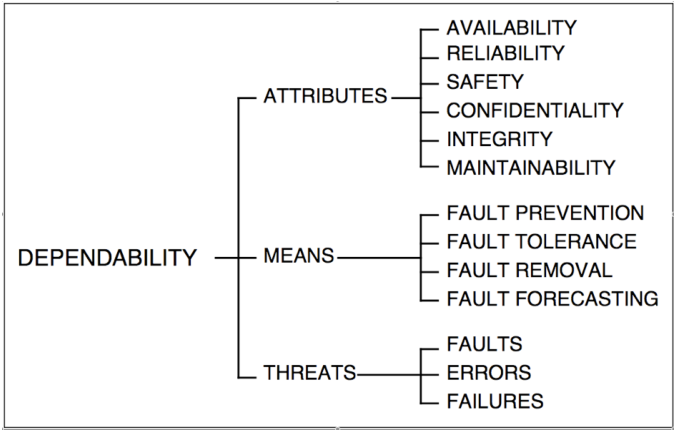
\includegraphics[width=0.60\textwidth]{images/dependability_tree.PNG}
	\caption{Dependability tree as defined by Laprie}
	\label{fig:dependability_tree}
\end{figure}

The attributes are the quality measures of a system. In this masters project, we will mainly analyze the availability and reliability attributes of OpenStack. Reliability is a measure for the continuity of a service, while availability measures the readiness for usage.\\

The dependability threats are system failures, system errors and system faults. A fault is the cause of an error, which is the system state that can then lead to a failure. The failure itself is an event that occurs when the service deviates from the specification. As a result, dependability threats can be seen as a chain, that can iteratively cause further faults, errors and failures through the layers of a system. We will present such dependability threat chains for the experiments we ran on OpenStack in Chapter~\ref{experiments}. \\

The means for handling the dependability threats and thereby improving the dependability attributes are fault prevention, fault tolerance, fault removal and fault forecasting. In fault prevention, the occurrence or introduction of a fault into the system is prevented. A fault tolerant system is able to provide the service as per specification even under faults. Fault removal is reducing the presence of faults in the system, and fault forecasting is estimating the number and consequences of faults. Regarding this masters project, we will look at the first three in relation to OpenStack.

\subsection{Applying Dependability to OpenStack}
When looking at the dependability of very complex systems such as OpenStack it is necessary to decompose the system and consider all layers individually. The bottom most layer we will consider is the infrastructure layer, i.e. the hardware of the nodes on which OpenStack is running and the network connecting them. On top, the OpenStack layer contains all OpenStack services, e.g., networking (Neutron), compute and visualization (Nova) or the identity service (Keystone). The top most layer that we will consider is the application layer, which is the applications on top of the OpenStack layer, e.g., services running on the virtual machines that are deployed on the OpenStack infrastructure. Figure~\ref{fig:depchain} shows an example of a dependability threat chain within the layers of an example OpenStack instance. 

\begin{figure}[h]
	\centering
		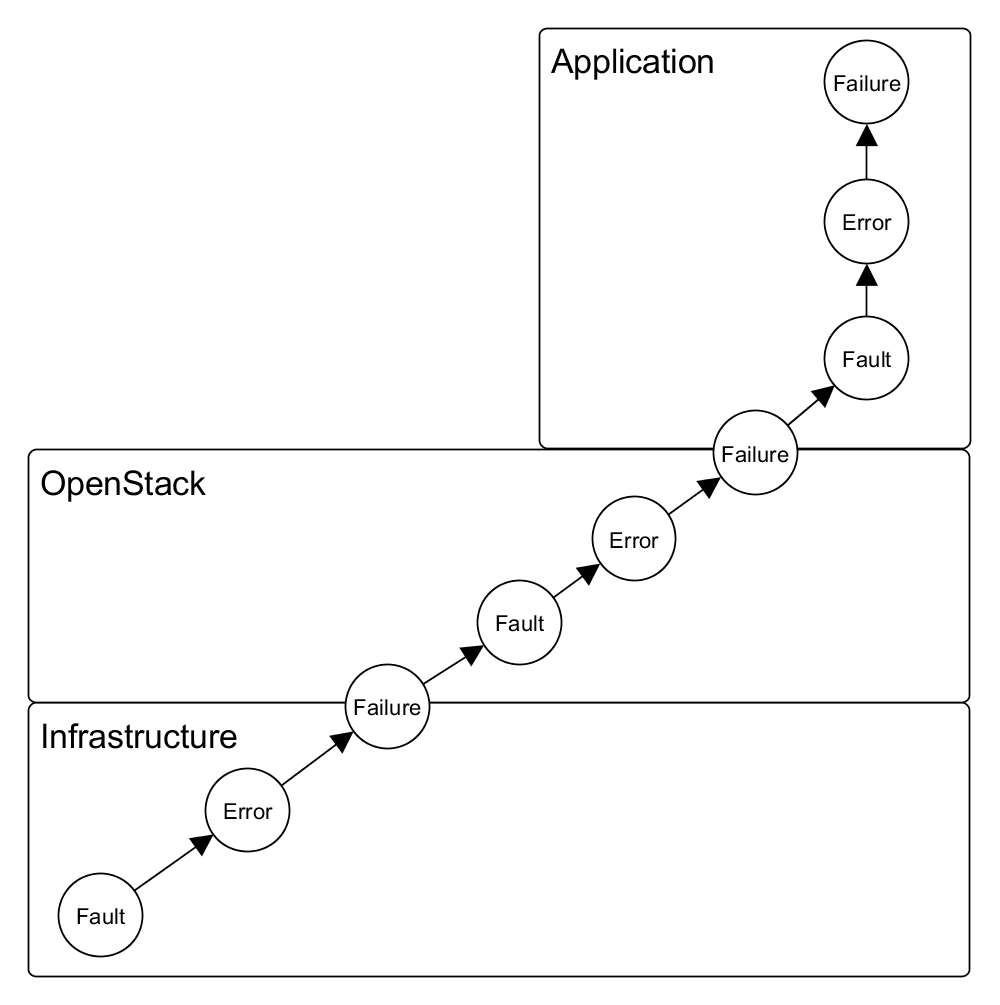
\includegraphics[width=0.60\textwidth]{images/depchain.PNG}
	\caption{Example dependability threat chain through layers of OpenStack}
	\label{fig:depchain}
\end{figure}

As one can see, a fault in a lower layer that leads to a failure can be propagated through the layers until it reaches the application, in which case the user will realize that the application is not running as specified.\\

OpenStack already provides measures of fault tolerance to prevent both system downtime and data loss. These measures are described in the OpenStack high availability guide\footnote{\url{http://docs.openstack.org/high-availability-guide/content/index.html}} for both active/passive and active/active setups. \\

An active/passive setup uses a separate service (such as Pacemaker) to monitor the actual OpenStack services and start passive resources when necessary. For OpenStack, stateless services like Neutron networking or the Glance object storage are suitable for active/passive high availability. \\

An active/active setup has multiple nodes running at the same time with the same services, when one fails over, the rest will take the load. In OpenStack, mainly the stateful services like the RabbitMQ message queue and the MySQL database will require an active/active setup. \\

With these dependability insights we were able to run dependability analysis on our OpenStack test environment. To do so, an OpenStack failure has to be specified. We define a failure of the OpenStack system with regard to the use case of downloading, uploading or streaming files from a virtual machine of a user. We then define a list of faults, that can cause the defined failure, and categorized them into virtual machine faults (server on VM not reachable, no network for VM, etc.), network faults (broken networking hardware, etc.), storage faults (broken hard drives, etc.) and OpenStack faults (Keystone crash, swift crash, etc.). The results of the experiments that test the dependability on the test environment will be described in Chapter~\ref{experiments}.\\

To conclude, with our master project system we are able to inject faults into our test environment and thus evaluate the fault tolerance of the OpenStack system. If the system thereby behaves in an unspecified manner, one is able to find possible bugs in OpenStack and if possible, one might be able to fix them, achieving a fault prevention this way. Over all, we draw insights about the reliability of OpenStack in relation to the test environment used in Chapter~\ref{experiments}.\\




%\newpage
\section[OpenStack Test Environment \texorpdfstring{{\textbf{\tiny \enspace (JE, SK, NK)}}}{}]{OpenStack Test Environment}
\sectionmark{OpenStack Test Environment}
\label{environment}
As described in Chapter~\ref{related}, we tried various possibilities to install an OpenStack system on a virtual environment. In this chapter we outline the challenges we faced with these possibilities, ultimately leading to the decision to create our own installation routine for a virtual OpenStack environment. Also, we will describe this test environment in detail.\\

\subsection{Existing OpenStack Installation Possibilities}
\label{installpossibilities}
We first tried installing the cloud computing environment HP Helion community edition. It promises an easy installation routine with little need for configuration. Further, it is possible to install HP Helion as an all-in-one system on virtual machines in addition to deploying it on bare-metal. This is an advantage with respect to our requirement of achieving a virtual test environment for reproducible test results. However, even though HP Helion has its advantages for setting up one's own IaaS system for a real use scenario, we came to the conclusion that it is not suitable for our needs. The installation of HP Helion took around 90 minutes on our hardware, which is not feasible for repeated installations. Further, we found that HP Helion does not survive a reboot of the host or the virtual machines it is running on. Fixing this issue would have required understanding the underlying installation scripts, which would still not have been beneficial in understanding OpenStack itself. Additionally, with our limited knowledge of HP Helion, it would have been a challenge to customize the system to fit our needs. We thus concluded that we would not use HP Helion for analyzing the dependability of OpenStack in line with this masters project.\\

A further option for an OpenStack deployment to work with for dependability testing we considered was DevStack. Due to the nature of the use cases for which DevStack is made, multi-node and high-availability setups are not the main focus, and therefore not documented well enough for us to customize DevStack and use it for dependability analyses. Also, it is not possible to generalize results of dependability analyses run on DevStack to a full OpenStack installation, as DevStack is not designed with real deployment in mind. As a result, we decided to use a full OpenStack installation for running our analyses.\\

\subsection{Specifying our own OpenStack Environment}
In order to be able to make the OpenStack test environment installation as easy and quick as possible, so that one can concentrate on the dependability analysis, we chose to install OpenStack virtually. A further advantage of this virtual installation is the reproducibility of experiment results, which is important to be able to make scientific statements about the dependability of OpenStack. We used libvirt\footnote{\url{http://libvirt.org/}} to create a number of virtual machines based on simple configuration files and Ansible\footnote{\url{http://www.ansible.com}} to orchestrate the installation of OpenStack on these nodes. The details of this automated installation are described in Chapter~\ref{installing}.\\

In order to create an useful test environment for dependability experiments, it was necessary to define an architecture. We chose this architecture to be a simplified OpenStack instance, meaning that we focus only the most important of the OpenStack services available. This can be seen as a bottom-up approach, as we focus on evaluating a simpler system than one might encounter when looking at an OpenStack system in production mode. One advantage of this approach is that, due to the simplicity, it is easier to make statements about OpenStack in general, than on one specific system. Libvirt and Ansible allow to add more nodes, create a more complex OpenStack system and, extend the proposed architecture by means of high availability mechanisms. We then draw conclusions about their effectiveness.\\

Figure~\ref{fig:arch} shows our virtual test environment architecture, which is the proposed architecture of the official OpenStack install guide\footnote{\url{http://docs.openstack.org/kilo/install-guide/install/apt/content/index.html}}. All nodes are virtual machines running on a physical host. The tenant virtual machines are dispatched on the compute node by means of nested virtualization. By default, our environment contains the following nodes:
\begin{itemize}
	\item One controller node: this node runs the OpenStack Dashboard (Horizon), the API services, the MySQL database, the RabbitMQ message queue server, the scheduler for the compute resources, Identity (Keystone) and Image (Glance) services.
	\item One network (Neutron) node: this node handles the internal and external routing and DHCP services for the virtual networks.
	\item Two compute nodes: the compute nodes are the computing resources for running the virtual machines of the OpenStack users. They run the hypervisor and services like \verb|nova-compute|, which is responsible for creating and terminating virtual machine instances through the hypervisor APIs.
	\item Two object storage (Swift) nodes: these nodes operate the OpenStack container and object services and each contain two local block storage disks for persisting the objects.
\end{itemize}

Further, the following networks are used to communicate between nodes and instances:
\begin{itemize}
	\item Management network: this network is used for the OpenStack administration, i.e., it connects the OpenStack services on the different nodes. 
	\item Tenant or tunnel network: these networks can be created by the OpenStack users to achieve communication between projects or instances. 
	\item External network: this network provides internet access to the instances.
\end{itemize}

This architecture is comprehensive enough to test various OpenStack use cases and analyze the dependability of the system.\\

\begin{figure}[h]
	\centering
		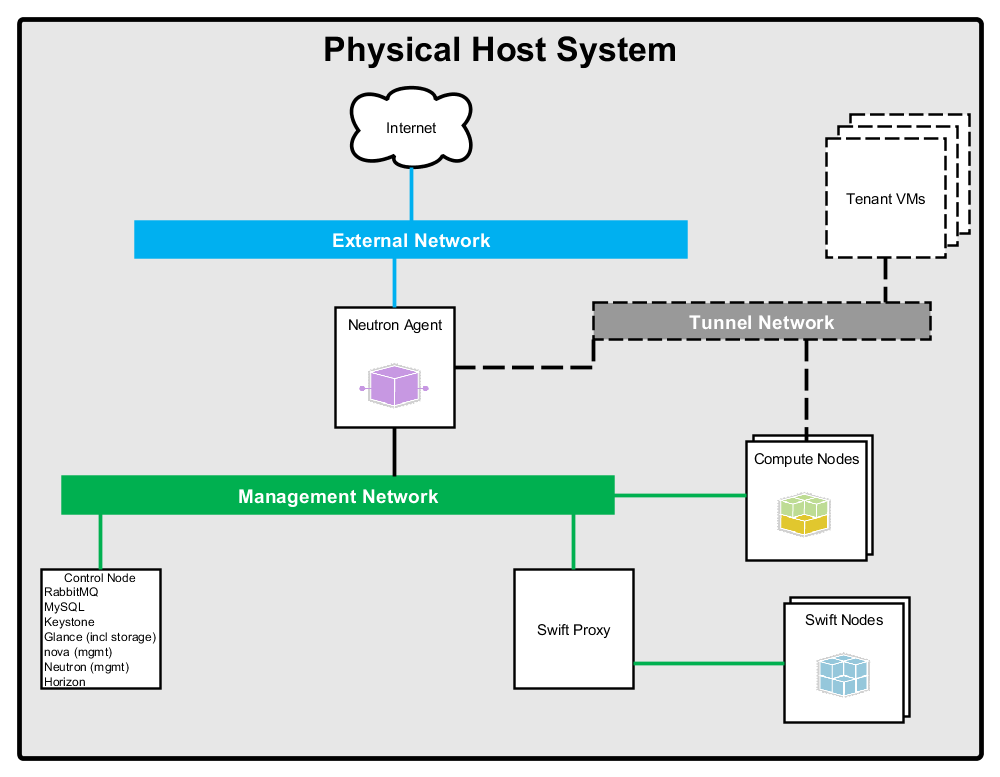
\includegraphics[width=0.90\textwidth]{images/architectureEN.PNG}
	\caption{Our test environment architecture}
	\label{fig:arch}
\end{figure}

The virtual OpenStack installation requires far less hardware resources than a distributed bare metal installation. It is possible to install a fully functional simplified test environment with one compute and object storage node on a quad-core Intel Xeon machine with 8GB RAM. For the full installation, more resources are recommended. We used a 16-core machine with 64GB RAM. 














%\newpage
\section[Automated Installation of OpenStack \texorpdfstring{{\textbf{\tiny \enspace (SK, NK)}}}{}]{Automated Installation of OpenStack}
\sectionmark{Automated Installation of OpenStack}
\label{installing}

In this chapter, we describe the automated installation process of OpenStack on our virtual environment. We give an introduction to the usage and a conceptual overview, however the the more technical aspects of the system are documented in higher detail in Appendix~\ref{appendix}.

\subsection{How to Install OpenStack using our System}
The installation scripts are developed and tested on a Ubunutu 14.04 LTE (Trusty Tahr) desktop version. All required dependencies (e.g., Ansible, libvirt, etc.) are installed automatically, thus an internet connection is required. The complete installation can be started by running the script \verb|install.sh|. It installs OpenStack virtually creating the architecture described in Capter~\ref{environment}. The virtual machines are automatically created. They can be managed using the virtual machine manager, which is also installed during the installation. After the successful installation (which will take ten to fifteen minutes) OpenStack Horizon can be reached at \url{http://controller/horizon/}. Default log-in credentials are demo/demo and admin/admin.\\

After the successful installation, a snapshot named ``initial'' is created. This allows for thorough dependability testing without re-installing the whole system after each experiment. Snapshots can be created manually as well: using the script 
\begin{verbatim}
snapshot_virtual_machines.sh <snapshot_name> 
\end{verbatim}
with \verb|<snapshot_name>| being the parameter for the name of the snapshot to be created. The snapshotting mechanism will shut down all virtual machines, snapshot the virtual hard drives of all nodes, and bring back up all machines.\\

To revert to a specific snapshot, the script \verb|restore_snapshot.sh| can be used. It will list all available snapshots, and revert all virtual machines back to the selected snapshot. Like taking the snapshot, reverting will also require the restart of the virtual machines.

\subsection{Creating the Virtual Environment}
\label{subsec:createve}
The virtual environment, i.e., the virtual networks and the virtual machines, are defined in the \verb|config| folder as libvirt network and libvirt domain XML-files. These XML-files define for example the IP addresses of the networks or the hardware specifications (size of RAM, number of cores, virtual hard drives, network interfaces) of the virtual machines. The virtual machines are then created with an Ubuntu cloud image\footnote{\url{https://cloud-images.ubuntu.com/trusty/}}, which are pre-configured images customized especially for running on cloud platforms. \\

The initialization of the virtual machines is done using cloud-init\footnote{\url{https://cloudinit.readthedocs.org/}}, which allows for setting passwords and SSH keys for easily connecting to the them afterwards, which is also a prerequisite for utilizing Ansible in the next steps. Further, using cloud-init, the correct \verb|etc/network/interfaces| configuration files are copied to the virtual machines. \\

In addition to the virtual machines for the OpenStack nodes, a further virtual machine named ``aptcache'' is created. This machine is used as a package repository by the others. The packages it delivers are not updated, meaning that the versions of all installed packages are frozen. This is important for acquiring a reproducible test environment and prevents different experiment outcomes to be caused by different package versions throughout the system.\\

These virtual machines create the base of the virtual OpenStack test environment and are now ready for the actual OpenStack installation.

\subsection{Installing OpenStack on Virtual Machines with Ansible}
In order to be able to install OpenStack on the created virtual environment, Ansible must be configured in such a way that virtual machines are grouped. This allows for installing different parts of OpenStack on the different nodes. These groups are defined in a so called Ansible hosts file, which assigns the IP addresses of the different nodes to different groups. In our case, each node type is a group, i.e., ``controller'', ``network'', ``compute'' and ``object''. This allows for the so called Ansible playbooks to be executed on the specified groups of nodes in parallel. \\

The Ansible playbooks that run the installation of OpenStack on the virtual nodes are strongly based on the official OpenStack installation guide\footnote{\url{http://docs.openstack.org/kilo/install-guide/install/apt/content/index.html}}, which is very extensive. This gives the advantage of not having to write any further OpenStack related documentation additionally to the documentation of the technicalities of the creation of the virtual machines and the Ansible installation. The arrangement of the Ansible playbooks in a folder structure derived from the content of the OpenStack documentation allows for easily finding the corresponding part of the documentation should one require information about a certain part of the installation.\\

The Ansible installation of OpenStack starts with an initial preconfiguration of the virtual nodes. In this step, the hosts files are created in order to be able to connect to the nodes by their host names. These host names are then also added to the SSH \verb|known_hosts| files to enable the SSH connection without warning messages. Further steps include setting the locale of the virtual machines to prevent locale errors as well as deactivating the \verb|/etc/cloud/cloud.cfg| file, as all configuration of the images is done in the previous step, see Chapter~\ref{subsec:createve}.\\

A special virtual machine named ``aptcache'' is set up first and independently of the others. It runs Apt-Cacher-NG\footnote{\url{https://www.unix-ag.uni-kl.de/~bloch/acng/}}, a caching proxy for Linux package repositories. All other VMs are set up to request their packages through it. This a) decreases network traffic and wait times and b) can be used to repeat the setup process while using the exact same package versions as the first time: The first install seeds the package cache, a repeated installation then can receive all packages from the cache instead of fetching potentially newer versions from upstream. To allow this, the cached data is not stored in the VM, but in a folder shared from the host machine.\\

The first step of the actual OpenStack installation is installing the basic environment. This includes adding the OpenStack package repository to the nodes and installing the MySQL database on the controller and the message queue RabbitMQ on all nodes.\\

The next step is the installation of the OpenStack identity service (Keystone) on the controller node. This service is responsible for the permissions of users and keeping track of the available OpenStack services with their endpoints. The installation of this service includes creating a database, installing the Keystone client packages and populating the database. A demo and an admin tenant are initially created. As with all OpenStack services, the installation is finalized by creating the service entity and the API endpoint.\\

Next, the image service Glance is added on the controller node. This service allows for retrieving and registering virtual machine images. Again, a database for this service is created along with the installation of the Glance client packages and the creation of an API endpoint.\\

OpenStack compute is then setup on the controller and the compute nodes. This component is responsible for the administration and hosting of the computing systems. It allows - among other things - for creating and terminating virtual machine instances through hypervisor APIs and is responsible for scheduling on which compute node an instance should run. To install the compute service Nova on the controller, the respective database and API endpoint is created and the nova service is configured. On the compute nodes, the nova-compute packages are installed and configured to run a QEMU hypervisor with the KVM extension.\\

The OpenStack networking Neutron components are installed next on the network, controller and compute nodes. The main responsibility of the networking component is to provide connectivity between the instances running on the compute node. On the controller node, database and endpoint API are created, the networking server component is configured and the Modular Layer 2 plug-in is configured. This plug-in is responsible for the networking framework of the instances running on the compute nodes. On the network node, the networking components are installed and configured accordingly. The layer-3 agent for routing services, the DHCP agent, the metadata agent and the Open vSwitch service are configured. Lastly, the networking components, the Modular Layer 2 plug-in and the Open vSwitch service are configured on the compute node. The external and tenant networks are then created to finalize the installation.\\

The OpenStack web interface dashboard Horizon is then installed on the controller node. This allows administrators and users to access and manage their resources on the OpenStack cloud.\\

The last component that is added to OpenStack in regards to this masters project is the object storage Swift. This allows to create containers, upload and download files and management of the objects on the storage nodes. On the controller node, the proxy service that handles the requests for the storage nodes is installed and configured. The storage nodes require two empty storage devices for persisting the objects. The virtual machines for these nodes contain two virtual devices in the qcow file format. The OpenStack Swift components are then installed and configured on the object storage nodes. Following the installation, the initial account, container and object rings are created.









%\newpage
\section[Running Dependability Experiments \texorpdfstring{{\textbf{\tiny \enspace (JE, SK)}}}{}]{Running Dependability Experiments}
\sectionmark{Running Dependability Experiments}
\label{experiments}
In this chapter, we will describe our OpenStack dependability experiments and their results. The implementations of these experiments all follow the same structure, so that it is easy to add further experiments if needed. In our experiments, we focused on covering the failure of various OpenStack components or nodes. We will give insights on how these failures affect the OpenStack environment and how the system deals with each fault. This serves partly to show weak points of the setup and partly to document details about its behavior.\\

Experiments consist of multiple stages: The \emph{setup} stage creates all elements necessary to run the experiment. The \emph{break} stage then breaks things. An optional \emph{heal} stage tries something simple to undo the damage (e.g. reboot a shutdown node). After each of this stages, a \emph{check} step is executed, which observes the state of the system and reports its findings to the user. Generally, after the setup stage all checks should be successful. Where user observations are useful (e.g. by looking not just at API results, but seeing how Horizon represents situations), the user is prompted to do so.\\

Using the snapshotting mechanism, the user can always completely restore the system, even if it didn't survive an experiment. This is not done by default because a) it takes some time and is not always necessary and b) to allow the user to inspect the system state after the experiment has concluded, e.g. to find or work out steps to fix remaining issues.

\subsection{How to Run the Experiments}

Experiments can be run by the shell script \texttt{run\_experiment.sh}. It lists the experiments and allows to run a specific one. It also allows to choose between different verbosity levels. The default verbosity \texttt{-v} shows a structured high-level overview with enough output to follow the experiment. \texttt{-vv} shows additional details and asks for confirmation between steps to give the user time to inspect system state manually if desired. The highest level \texttt{-vvv} shows all the output generated by commands in the experiment. This is useful to understand the how the experiment works and to debug potential issues during experiment development.\\

Internally, each experiment has a script \texttt{run.sh} that launches the individual steps, which live in specially formatted scripts of their own.

\subsection{Experiment Results}
This section describes our four example experiments and discusses their results. 

\subsubsection{Experiment 1: Control Node crash}
In this experiment, a crash of the control node in the system is simulated. \\

\textbf{Technical Background}\\
The controller node stores global information of the OpenStack cluster and runs the sub-services depending on it, which then give services on other nodes the specific information they need to e.g. run a specific instance or to build network connectivity. In our setup, it also provides the dashboard Horizon and runs the authentication service. A failure of this node obviously is going to have a large impact, but some things that already are set up on other nodes continue to operate.\\

\textbf{Experiment}\\
The experiment script creates an instance and then uses ping to verify availability of both the compute node and the started instance. It also tries to access OpenStack APIs. To simulate the fault, it either issues a shutdown command, simulating the unavailability of the node to the controller or more severely, just turns off its infrastructure virtual machine to simulate a full crash.\\

\textbf{Results and Conclusion}\\
While the control node is turned off, outside connectivity to the already created instance remains, since it runs on the compute node and its network connection to the outside (managed by Neutron, via the network node) is unaffected. On the other hand, all attempts to use OpenStack APIs fail. Most user-facing APIs are accessed via the controller and thus completely unavailable. Others report errors, since every action has to be authorized using the Keystone service, which only runs on the compute node in our setup.\\

After the controller node is up again, OpenStack takes a few minutes to reestablish all service connections and in most cases is fully operational again. It is possible that the compute instances fail to reconnect to RabbitMQ and their services have to be restarted manually\footnote{\url{http://docs.openstack.org/openstack-ops/content/maintenance.html\#cloud_controller_storage}}. \\

This shows that already running instances on OpenStack are generally not impacted by temporary failure or maintenance of quite a few central OpenStack components, but during their inavailability no changes can be made and recovery might need manual intervention by an operator. \\

If the controller node was shut down hard, obviously many more failure scenarios related to the underlying operating system or services are possible, e. g. missing information in databases or damaged file systems.\\

\subsubsection{Experiment 2: Memchached Service Loss of Data}
This experiment shows the effects of Keystone losing authentication tokens due to the design of its storage mechanism.\\

\textbf{Technical Background}\\
A common way to authenticate for operations against the OpenStack API is to use tokens. A more complex and privileged authentication (e.g. a passsword check) is done once to obtain a security token. These tokens have a limited lifetime and can be limited in scope, so a user can generate a token for a specific task and pass it to a service, which then can use it to access other services in the users name. Tokens also are internal to OpenStack, whereas other authentication might require accessing an external authentication provider (e.g. an LDAP server).\\

The Keystone service stores these tokens in memcached\footnote{\url{http://memcached.org/}}, which is, as the name alludes to, an in-memory caching service. Designed as just a fast caching layer, it neither has persistence to disk nor does it guarantee to keep all data it stores. If it deems necessary it can evict any information at any time (i.e. because it is under memory pressure).\footnote{\url{https://code.google.com/p/memcached/wiki/NewUserInternals\#How_the_LRU_Decides_What_to_Evict}}\\

\textbf{Experiment}\\
The admin credentials are used to create a token. To verify the tokens validity, it is used to authenticate an operation against the Keystone API. To cause memcached to evict it from the cache, the command for memcached to delete all its data is issued. \\

\textbf{Results and Conclusion}\\
Subsequent attempts to use the token fail, since it has been deleted. This shows the consequences of OpenStack using an unreliable data store to save a central element of its authentication system, instead of using memcached as designed only as a cache to improve lookup speeds. \\

If a user is  logged into the Horizon dashbord while the experiment is running, it also sometimes allows to observe failures: The dashboard site is still accessible (because the session on the web server still exists), but no information from OpenStack is shown because attempts to retrieve it fail due to the invalid token. The user has to log out and back in again to create a new token. 

The implementation of this experiment is described in Appendix~\ref{a:memcache}

\subsubsection{Experiment 3: Compute Nodes Unavailable}
This experiment documents the behavior if connectivity to compute nodes is lost.\\

\textbf{Technical Background}\\
Instances are distributed among the compute nodes by the Nova scheduler, which runs on the controller node. Inspecting the state of VMs, e. g. directly via the Nova API or via the Horizon Dashboard is also done via information stored by Nova on the controller node, where it collects information from all compute hosts.\\
If the controller looses connectivity to compute nodes, it can't accurately report the state of individual instances, as seen in this experiment. \\

\textbf{Experiment}\\
This experiment first creates an instance to observe throughout the different stages. Then the first level of fault is introduced: All compute nodes are removed from the management network. Then an attempt to start a second instance is made. After this, a more severe fault is created by shutting down all compute nodes. Then a "fix" is attempted by restarting the VMs.\\

\textbf{Results and Conclusion}\\
After the first fault,  Nova on the controller has no connectivity to the compute nodes and is therefore unable to actually start the second instance. The first instance is still reported as being active, which in this case is correct: it is still running and can be reached from the outside network. Since it already has lost all connectivity to the compute nodes, things look exactly the same after the compute nodes are actually shut down, but in this case the state information is wrong: the VMs obviously are not active, but shut down together with the host they were running on. After the reboot of the compute nodes, they reconnect to the controller and the state of all VMs is reported correctly again.\\

This shows that when Nova looses connectivity to a compute node it can't report accurate information, which is one of the reasons why Nova doesn't implement functionality to automatically restart such VMs.  Short interruption of Nova services, e.g. due to software updates, do not necessarily disrupt instance operations. Such decisions are left to other systems that can collect more information (e.g. by running active tests against VMs) and can be configured for specific application needs, like OpenStack Heat. \\

We find it interesting that the developers choose to report such instances as active and did not introduce another state to represent this special situation.

\subsubsection{Experiment 4: Object Storage Crash}
In this experiment, the crash of object storage (Swift) nodes is simulated. The experiment is setup by uploading a 100 MB test file to the fully functional object storage cluster, consisting of two object storage nodes. \\

\textbf{Technical Background}\footnote{Detailed information on OpenStack Swift is given in \cite{swift} or on \url{https://swiftstack.com/openstack-swift/}}\\
OpenStack Swift stores the copies of the same data on different nodes to prevent the loss of data in case of failure and to be able to offer massive scalability. As opposed to, e.g., a simple file system, Swift is an eventually consistent storage system. Objects in Swift are stored in containers, which contains meta data about the objects. Containers themselves are contained in an account, which is the storage area. The processes that run on a storage node thus are composed of account, container, object and proxy server processes. The proxy server is responsible for the verification and handling of API requests, as well as for deciding which node to send the request to. This includes choosing a substitute storage node, should the primary one be unavailable. To ensure consistency of the data across the nodes, a Swift auditor service continually checks for malformed data on the disks and moves corrupted objects into a specified quarantine. Replicator services check the hashes of the copies of objects on other nodes, and send out their respective copy of the object should it be inconsistent.\\

Regarding the architecture of the storage cluster, it can be divided in nodes, regions and zones. Our system runs two storage nodes with one region and zone, as described in the OpenStack documentation we base our system on. Regions represent geographically separated parts of the cluster, and zones separate physical hardware, i.e. different racks. Our storage nodes contain two storage disks each. Swift partitions storage disks into partitions (which in OpenStack indicate rather a directory than a conventional storage partition), the maximum number of which can be configured - in our case $2^{10} = 1024$. These partitions are replicated as uniquely across the cluster as possible a specified number of times. In our system, three replicas are created. The replicas are mapped to the partitions in a hashing ring. \\

\textbf{Experiment}\\
The experiment contains multiple steps. Aim of the experiment is to verify the availability of a test file download even after the crash of a storage node. Due to the fact that each node has two storage disks, and three replicas of each object are configured, the test file is replicated on one node twice, and on the other once. After the upload of the 100 MB test file, it is downloaded to verify the functionality. Next, a crash of one of the object nodes is simulated. Again, the download is initiated before the node is restarted. This procedure is then done for the simulated crash of the other storage node. In a last step, the crash of both nodes is simulated.\\

\textbf{Results and Conclusion}\\
The results of this experiment show that, for a correctly setup and configured OpenStack system with two storage nodes, a storage node crash will not impair the functionality for the user. The test file object is replicated correctly amongst the nodes, i.e., one node contains two replicas (one on each hard drive), and the other contains one replica. This is due to the fact that Swift tries storing replicas in the most unique way possible amongst the cluster. Only when both storage nodes fail will the download of the test file be impossible. This is an obvious trivial test case that was added to the experiment for completeness.\\

The number of replicas is crucial for Swift to be able to cope with a storage node crash. Three replicas is a configuration that is found often when applying redundancy to high availability systems. However, two replicas would also suffice for surviving a storage node crash in our setup, as Swift distributes the replicas in the most unique way possible, which would assign both nodes one copy of the test file. 







%\newpage
\section[Conclusions and Future Work \texorpdfstring{{\textbf{\tiny \enspace (JE, SK, NK)}}}{}]{Conclusions and Future Work}
\sectionmark{Conclusions and Future Work}
\label{conclusion}

In our masters project we created a platform for the automated installation of an virtual OpenStack environment as well as a framework for some first dependability experiments on this environment. The advantage of our platform is the very fast installation (ten to fifteen minutes) of a complete OpenStack environment on very limited hardware compared to a full bare metal installation. This makes running dependability experiments comparatively easy. Features like snapshotting would not be available on a bare metal setup, but are very useful when repeating such experiments. Further, our platform is easily extendable, both for adding further OpenStack components as well as further experiments.\\

These features can be the foundation for future work. Due to the limited time and personal resources, we were not able to implement the installation of a full OpenStack high availability setup. Such a setup could make it possible to compare the dependability of the ``normal'' OpenStack setup to the high availability one, by running the experiments on both. Further, due to the fact that we use Ansible for the installation, the playbooks themselves can be easily used for installing OpenStack on bare metal. For this, the scripts for configuring the virtual environment could be extended in order to make it possible to configure a bare metal setup. This would allow running the experiments on a bare metal OpenStack installation.


%\newpage
%\printglossaries


%% Anhänge
%Hier kommt das Literaturverzeichnis
\newpage
\phantomsection
\addcontentsline{toc}{section}{References} % Zeile für das Inhaltsverzeichnis
\bibliographystyle{alpha}
\bibliography{bibfile}

\newpage
\begin{appendix}
\section{Code Documentation}
\label{appendix}
In this appendix we will document the technical aspects of the framework we created for the installation and evaluation of the OpenStack system.



\subsection{Folder Structure}
\begin{itemize}
	\item \verb|/|: This folder contains the most important scripts.  
	\item \verb|installation|: This folder contains various bash scripts that prepare the host machine as well as create and prepare the virtual machines for the OpenStack installation. The file \verb|install.sh| is the main file which is executed for starting the complete installation of the system. Snapshots of the current environment status can be taken with
\begin{verbatim}
snapshot_virtual_machines.sh <snapshot_name> 
\end{verbatim}
with \verb|<snapshot_name>| being the parameter for the name of the snapshot to be created. The snapshotting mechanism will shut down all virtual machines, snapshot the virtual hard drives of all nodes, and bring back up all machines. To revert to a specific snapshot, the script \verb|snapshot_revert.sh| can be used. It will list all available snapshots, and revert all virtual machines back to the selected snapshot. Like taking the snapshot, reverting will also restart the virtual machines.
	
	\begin{itemize}
		\item \verb|installation/config|: This folder contains all files needed for configuration of the OpenStack installation. The file \verb|installation_configuration.sh| will allow for changing default passwords, URLs, IP addresses etc. The folder
\verb|ansible| contains the Ansible configuration file and the hosts file, which defines the hosts (i.e. which IP address maps to which type of node) and needs to be customized when adding/removing nodes. The \verb|network| folder contains the .xml files that specify the three virtual networks created by libvirt. A folder called \verb|vm| contains for each virtual machine that is to be created a folder with the name of that VM. In the VM folder itself reside four files: \verb|creation.xml| defines the hardware of the respective VM to be created by libvirt. \verb|etc_network_interfaces| contains the \textbf{/etc/network/interfaces} file of the respective VM.
	\end{itemize}
	
	\begin{itemize}
		\item \verb|installation/playbooks|: This folder contains all the playbooks that set up OpenStack on the virtual nodes. The containing folder structure is based on the available documentation of OpenStack Kilo\footnote{\url{http://docs.openstack.org/kilo/install-guide/install/apt/content/}}, which is also contained as 
\begin{verbatim}
openstack-install-guide-apt-kilo.pdf
\end{verbatim}		
		in the top hierarchy of the folder structure.
	\end{itemize}
	
	\begin{itemize}
		\item \verb|installation/tools|: this folder contains further bash scripts that provide various general reusable functionalities for the installation of OpenStack.
	\end{itemize}
\end{itemize}




\subsection{Creation of Virtual Machines}
To create the virtual machines, several steps have to be completed, which will be described here. A failure in one step results in the following steps to be aborted, as to prevent faulty installations.


\subsubsection{Installation of tools}
\texttt{install\_tools.sh} installs packages and tools that are required for the bash scripts or the user, such as the virtual machine manager or Python's jinja2\footnote{\url{http://jinja.pocoo.org/docs/dev/}} library, which is used by Ansible and other scripts to instantiate templates.\\

\texttt{install\_ansible.sh} installs Ansible, which is used in later steps to install the OpenStack components on the virtual machines.\\

\texttt{install\_lib\_virt.sh} installs libvirt which is used to manage the virtual machines. Libvirt is installed in the correct order along with qemu-kvm.


\subsubsection{SSH Keys}
\label{ssh-keys}
Ansible requires SSH to be used to connect to the virtual machines. We chose to use public/private key authentication. This allows for an easy log-in on the virtual machine without requiring a password for each machine. \texttt{create\_ssh\_keys.sh} creates the SSH keys on the host system. These keys are added as trusted keys to the virtual machines. Thus, a log-in with \texttt{ssh ubuntu@controller} enters the shell on the controller host without any further authentication.

\subsubsection{Networks}
The virtual machines are connected by several networks. The network configuration is defined in the \texttt{config/network} folder as libvirt XML files. \texttt{create\_virtual\_networks.sh} creates the virtual networks using libvirt.


\subsubsection{VM Images}
\texttt{create\_virtual\_machine\_image.sh} creates the images for the virtual machines. As configured in the \texttt{installation\_configuration.sh} an Ubuntu cloud image is downloaded. This image serves as the basis for all future virtual machines. \\

Since each virtual machine serves a certain purpose, the images need to be configured individually. \texttt{create\_virtual\_machines.sh} uses the downloaded image and adapts it. The configuration for each vm is listed in the \texttt{configuration/vm} directory. Such a directory includes several template files:

\begin{itemize}
	\item \texttt{etc\_network\_interfaces} is the file that contains the network configuration that is then stored in \texttt{/etc/network/interfaces} on the virtual machine.
	\item \texttt{user-data.cloud-config} defines the configuration of the virtual machine, including passwords, host-names, the trusted SSH keys from Section~\ref{ssh-keys} as well as the network interfaces file.
	\item \texttt{creation.xml} contains the libvirt definition of the virtual machine. This includes the virtual hard-drives, the network interfaces and virtual input/output devices.
\end{itemize}

These template files are instantiated using the jinja2 syntax. The variables origin from the virtual machine configuration as well as the \texttt{installation\_configuration.sh}, in which all installation relevant parameters can be adjusted. \\

After the virtual machines have been defined, they are started. \texttt{wait\_for\_virtual \_machines\_to\_start.sh} starts the virtual machines and waits for the respective SSH port to open. Once the virtual machine is started, its public SSH key is copied into the known hosts file to allow an SSH connection without prompting for verification of the key. This allows for a more fluent installation process.


\subsubsection{Configuration of Ansible}
The \texttt{installation\_configuration.sh} should be the first and only place to make configuration changes. Also, Ansible is used for further modification of the virtual machines. As a consequence, the configuration variable definitions need to be accessible to Ansible. \texttt{configure\_ansible\_for\_vms.sh} copies the variable definitions into the corresponding Ansible files. \\

Ansible uses a hosts file which categorizes all computers that shall be reached. This template file is instantiated and copied to the \texttt{/etc/ansible} directory. \\

The Ansible configuration contains the user-name that is used to log into the virtual machines via SSH. This configuration file is also copied to \texttt{/etc/ansible}. \\

\texttt{installation\_configuration.sh} contains variables used by the Ansible scripts. These variables are formatted and copied into an Ansible playbook, which is located at \texttt{/etc/ ansible/roles/config/vars/main.yml}. This means whenever the role ``config'' is used in an Ansible playbook, all variables from \texttt{installation\_configuration.sh} can be used. Additionally, environment variable sets ``demo'', ``admin'' and ``token'' are specified, which can be used to authenticate against OpenStack's Keystone later on in the installation process. 





\subsection{OpenStack Installation with Ansible}
As stated before, we follow the structure of the OpenStack documentation\footnote{\url{http://docs.openstack.org/kilo/install-guide/install/apt/content/index.html}} for the Ansible\footnote{\url{https://docs.ansible.com/ansible/index.html}} playbooks. Ansible is an orchestration tool that allows for configuring and managing groups of nodes simultaneously. For example, it is possible to run commands, change files or restart services on the remote machines. Ansible comes with a variety of useful modules, that allow extremely complex tasks, such as editing .ini files\footnote{Ansible makes editing .ini files extremely complex, as it uses the python .ini file parser.}.\\

Ansible playbooks are written in the YAML syntax, which basically define a list of commands. The playbooks as well as the commands in them have a name, which is displayed in the terminal when the playbook is run, making it easy to follow current progress or see where an error might have occurred. A parameter \verb|hosts| in each playbook allows for specifying on which nodes the playbook will run, as specified in a Ansible hosts file, which maps all node's IP addresses to their specific groups. The output of a running Ansible playbook is shown as follows:
\definecolor{terminalgreen}{rgb}{0.25,0.54,0.02} 
\definecolor{terminalorange}{rgb}{0.77,0.63,0}
\begin{Verbatim}[commandchars=\\\{\}]
\color{darkgray}PLAY [Basic environment > OpenStack packages > add OpenStack repository]

\color{darkgray}TASK: [1. update the cache] ******************************************** 
\color{terminalgreen}ok: [192.168.100.31]
\color{terminalgreen}ok: [192.168.100.11]
\color{terminalgreen}ok: [192.168.100.51]
\color{terminalgreen}ok: [192.168.100.21]

\color{darkgray}TASK: [2. install cloud keyring] ***************************************
\color{terminalorange}changed: [192.168.100.31]
\color{terminalorange}changed: [192.168.100.21]
\color{terminalorange}changed: [192.168.100.51]
\color{terminalorange}changed: [192.168.100.11]

\color{darkgray}TASK: [3. add repository] **********************************************
\color{terminalorange}changed: [192.168.100.31]
\color{terminalorange}changed: [192.168.100.21]
\color{terminalorange}changed: [192.168.100.11]
\color{terminalorange}changed: [192.168.100.51]
\end{Verbatim}
This is the output generated by the playbook 
\begin{verbatim}
02_basic_environment/05_OpenStack_packages/
                     01_enable_the_OpenStack_repository.yml
\end{verbatim}
which corresponds exactly to the Chapter 5 Section 1 in the OpenStack documentation\footnote{\url{http://docs.openstack.org/kilo/install-guide/install/apt/content/ch_basic_environment.html\#basics-packages}}.\\

Ansible allows for using variables in the playbooks for central configuration management. 

\subsection{Snapshots}
The whole installation process takes about ten to fifteen minutes. It is not advisable to re-run this process every time an experiment starts. Therefore, snapshots can be created. Once the installation process finished, a snapshot ``initial'' is created, using \texttt{snapshot\_virtual\_machines.sh}. After each experiment, one can revert all the virtual machines to this snapshot, using ``restore\_snapshot.sh''.\\

The libvirt snapshotting mechanism is not fully implemented yet. Libvirt is capable of taking two main types of snapshots: external and internal. An internal snapshot allows the changes of a virtual machine to be stored in a single qcow file. External snapshots store the snapshot itself in one file, but the changes are stored in an extra file. As of September 2015, external snapshots could be taken by libvirt, but not reverted\footnote{\url{http://wiki.libvirt.org/page/I_created_an_external_snapshot,_but_libvirt_won't_let_me_delete_or_revert_to_it}}. Thus, the OpenStack virtual machines are snapshotted internally, for which it is necessary that all virtual machine storage devices are in the qcow format.




\subsection{Dependability Experiments}

In this project we created four dependability experiments as described in Chapter~\ref{experiments}.

\subsubsection{Inner Workings of the Memcache Flush Experiment}
\label{a:memcache}

This experiment has four steps. If one step fails unexpectedly the following steps are omitted to allow examination of the underlying problem. \texttt{run.sh} runs the whole experiment, setting environment variables, too. The logging level can be changed by passing \texttt{-vv} or \texttt{-vvv} to it.\\

We want to create a token using OpenStack. Since we setup Ansible ssh, we can use \texttt{ssh ubuntu@controller} to connect to the controller. There, we can issue a token using \texttt{openstack token issue}. Shell scripts do not allow to change variables in other, running shell scripts. Therefore, the variable containing the token is saved to a file. This file is sourced by all scripts with updated variables. The token is created in the setup step.\\

After the token is created, we want to check that we can use it. \texttt{run\_checks.sh} sends a request to \url{http://controller:5000/v3/auth/tokens} to authenticate with the token. After setup this works and a new token is created.\\

Depending on the logging level of \texttt{run.sh} we are asked to review the output. \\

The second phase of the experiment begins with injecting the fault. 
Again, we can use ssh to connect to the controller and flush the memcache. This is dene on \texttt{break.sh}.

After this, we run the \texttt{run\_checks.sh} again and expect different output. Injecting the fault altered the system, made the memcache forget about the tokens previously issued. Thus, no new token can be created.

Since this experiment's fault is only temporary, there is no need to heal the system again. Other experiments would call a \texttt{heal.sh} to ensure proper operation of OpenStack after the experiment.

\subsubsection{Output of the experiments}

Each experiment has a file named \texttt{example\_output.txt}. It can be used as a reference. Here we show the output of the Memcache Flush experiment. It shows that a token can not be created using a token issued before the flush of the cache.

\definecolor{terminalgreen}{rgb}{0.25,0.54,0.02} 
\definecolor{terminalorange}{rgb}{0.77,0.22,0}
\begin{Verbatim}[commandchars=\\\{\}]
mpos2015-source$ ./run_experiment.sh 02_memcache_flush
+ Flush Memcache
  * SETUP
    - on controller, get token from Keystone (as admin)
  * Running checks
    - attempting to create new token using first token
    - token
      \color{terminalgreen}OK! Token created.
X-Subject-Token: 36e737434cc446a7a3d9ab95e9746cb9
  * CREATING FAULT
    - flushing memcache on controller
  * Running checks
    - attempting to create new token using first token
    - token
      \color{terminalorange}ERROR! No token created.
\end{Verbatim}


\subsubsection{Creating Dependability Experiments}
Dependability experiments can easily be created and added to the existing ones. All experiments consist of five main bash scripts, that dictate the structure of the experiments. These files need to be implemented when adding a new experiment.\\

Each experiment owns a main \verb|run.sh|, which is the entry point of the experiment. In this script, first \verb|setup.sh| is called, which contains all commands for setting up the OpenStack environment for the experiment, e.g., uploading files, getting tokens etc. \verb|break.sh| then causes the necessary failure in the OpenStack system, e.g. crashing a node or service. \verb|run_checks.sh| then asserts if the OpenStack system has survived the failure, running all necessary tests to test correct operation. Lastly, \verb|heal.sh| then restores any crashed nodes and brings the system back up to a running state (e.g., by reverting a snapshot if necessary), ready for the next experiment.




\subsection{Workarounds for Bugs}
We will describe some workarounds we used for some common issues we encountered to clear up any confusion that might arise else wise.
\begin{itemize}
	\item Module \verb|ini_file|: Due to the fact that Ansible is still under active development, some modules do not work as expected. The module \verb|ini_file| is used for editing .ini files. It contains a bug for .ini files containing a \verb|DEFAULT| section. We used a workaround to achieve correct editing of .ini files with a \verb|DEFAULT| section: at the beginning of the editing process, the section is renamed to \verb|DEFAULT_WORKAROUND|, then changes are applied, then the section is named back to \verb|DEFAULT|. This will result in correct .ini files.
	
	\item Segmentation fault: If a segmentation fault error is thrown during the installation process, this can usually be fixed by assigning the respective VM more RAM.
\end{itemize}








\end{appendix}
}
\end{document}
